\begin{otherlanguage*}{brazil}

\section{Playsound}

O desenvolvimento da plataforma Playsound.space começou durante o meu período de estágion o Centre for Digital Music (C4DM) na Queen Mary University of London (QMUL)\footnote{O Estágio aconteceu de junho de 2017 a maio de 2018 e foi financiado pelo Programa de Doutorado Sanduíche da CAPES}, onde tive a oportunidade de participar do grupo de pesquisa ligado ao projeto Audio Commons\cite{Font2016}. Depois de desenvolver o projeto Banda Aberta, o desejo era de trabalhar no desenvolvimento de um sistema que pudesse ser utilizado como um instrumento musical, que fosse capaz de produzir uma gama rica de sonoridades e não mais somente uma plataforma para tocar sons pré determinados. 

A iniciativa Audio Commons visa trazer conteúdo sonoro em Creative Commons (CC) para artistas e indústrias criativas. Licenças CC fornecem uma maneira padronizada para dar permissão ao público no compartilhamento e utilização de trabalho criativo em condições definidas pelos criadores de conteúdo, que pesquisa formas de aproveitamento e utilização de serviços online de distribuição de conteúdo sonoro com licenças em Creative Commons footnote{\url{https://creativecommons.org/}}. O projeto é financiado pela união Européia e tem entre seus obetivos, desenvolver uam ontologia para sons, e criar um mecanismo mediador para pesquisar sons de diversas fontes como as bilbiotecas Freesound.org, um grande repositório de samples; Europeana.org, que reúne um acervo de gravações históricas de diversas intituições européias e Jamendo.com, que reúne músicas novas produzidas em licensas livres.


Nosso principal domínio de aplicação é a improvisação musical que é definida como uma atividade musical autônoma \cite{Canonne2016} que geralmente leva a situações pluralistas, com ênfase no processo de tocar, e na iteração musical no momento \cite{BERGSTROEM-NIELSEN2016}. Em oposição à improvisação idiomática, como aquela praticada em algumas formas de jazz ou hip-hop, a improvisação livre pode levar à formas não metrificadas e sem escala ou tonalidade pré-determinadas, onde muitas vezes a variação de timbre prevalece\cite{Barthet:11a}. Já vinha desenvolvendo atividades em improvisação livre anteriormente, mas depois do início do doutorado, tive oportunidade de participar da Orquestra Errante, grupo conduzido pelo professor Rogério Costa que ensaia semanalmente no estúdio do NuSom na Universidade de São Paulo. 

Durante as práticas de improvisação musical que participei até agora, encontrava algumas dificuldades em utilizar softwares tradicionais como DAW patchers. Uma delas é de que muitos softwares do tipo DAW são baseados em grids temporais fixos, ou seja, existe um tempo que determina o fluxo dos acontecimentos sonoros, e embora esse tempo possa ser mudado, a estrutura rígida conflita com a necessidade da liberdade na improvisação. A estrutura em grade ou se impõe para os demais músicos, como um metrônomo, ou entra em conflito com os demais participantes. Além disso, as estruturas temporais também dificultam a criação de polirritmias. 

Softwares que se comportam como instrumentos virtuais, por outro lado, como sintetizadores e \emph{samplers} são mais fáceis de serem empregados na prática. Por serem baseados em gesto, o controle do fluxo sonoro fica a cargo do musicista, dependendo aí do tipo de controlador que ele usa, de sua expertise técnica em tocar, e da capacidade de variação timbrística do instrumento. No caso dos sintetizadores, as possibilidades de variação de sonoridade são constringidas pelos timbres oferecidos pelo fabricante ou programador, e em geral restritas a sons musicais, dentro de uma escala pré-determinada. Além disso, para se obter um bom controle de dinâmica, é recomendado a utilização de controladores externos, como teclados midi, por exemplo. Minha idéia era desenvolver algo que pudesse ser tocado em tempo real, e que permitisse mais variação sonora do que os softwares e ferramentas disponíveis no mercado.

No Contexto de novas interfaces para produção musical uma série de abordagens diferente têm sido desenvolvidas para o emprego do computador como instrumento musical na prática de improvisação livre. Exemplos incluem \emph{live coding} \cite{freeman2011collaborative} e orquestras de laptop \cite{Albert2012}. \emph{Live Coding} colaborativo ao vivo frequentemente envolve o desenvolvimento de tecnologia pra sincronização entre dispositivos \cite{Wilson2014}, que aqui não foi adotada devido à escolha estética de deixar a estrutura rítmica livre.


A ideia de tocar com uma ``paleta de sons expandida'' tem sido explorada na música desde Luigi Russolo  \cite{Merz2013} e especialmente depois da música concreta. A digitalização e a disponibilização de sons online potencializa essa ideia, como aponta Schnell:
\begin{citacao}
``In the age of digital sound databases and online music publishing services, the total disembodiment of digital sound turns into the promise of perpetual reincarnation of digital sounds through their permanent exchange and transformation."\cite{Schnell2013}
\end{citacao}

Nos instrumentos que funcionam a base de amostras de sons (samplers), as possibilidades sonoras são ampliadas pela possibilidade de utilização de sons não-musicais, ou em outras escalas, mas são dependes de se ter acesso e conhecimento de uma biblioteca grande de sons. Localizar samples em tempo real durante uma improvisação musical pode ser desafiador\cite{Xambo2018}, principalmente porque a improvisação exige do musicista uma reação espontânea e instantânea em tempo real \cite{canonne2011model}. Isso exige que o performer conheça bem e previamente os sons de uma determinada coleção, o que se torna impraticável se a coleção de sons é muito grande. Para contornar este problema, os praticantes normalmente selecionam uma amostra reduzida de sons, o que acaba também por reduzir suas possibilidades criativas durante as performances.

A digitalização do som, em conjunto com tecnologias Web e bancos de dados de áudio digital abre muitas possibilidades critativas, que como Schnell aponta, pode levar à ``promessa de reencarnação perp´tua de sons digitais através da sua permanete troca e transformação'' \cite{Schnell2013}. A utilização de amostras de sons pré-gravados é largamente empregada em uma série de tradições estéticas musicais como no emph{Hip Hop, Plunderphonics, Música Eletrônica, Música Concreta, composição de Paisagens Sonoras}. Bibliotecas online de áudio como Freesound.org, Redpanal.org, Sampleswap.org entre outras são utilizadas por compositores e produtores musicais de vários tipos de aplicações multimídia como cinema, publicidade, video games, e composições musicais \cite{Roma2013}. 

Alguns projetos desenvolvidos recentemente têm também esse norte como paradigma. O projeto API Cultor, por exemplo \cite{Ordiales2017} usa técnicas de \emph{machine learning} para prover um ambiente para re-utilização de sons de blibliotecas online. Lee et al. propõe uma ferramenta para \emph{live coding} com a API do Youtube para improvisação livre \cite{Lee}. Ao prover acesso a seu banco de dados por uma REST API \cite{Akkermans2011}, o site Freesound.org permite que musicistas e designers criem aplicativos que explorem seu conteúdo online para utilização ao vivo. BeatPush \cite{Feenstra2016}, é um exemplo de sequenciador usando esta API e o Freesound Explorer \cite{Font2016}, por exemplo, organiza os sons em uma configuração espacial por similaridade e usa cores para representar aspectos timbrais, no entanto, é uma aplicação mais voltada para navegação e exploração do que para tocar em tempo real, e não permite que os usuários selecionem sons a partir de buscas múltiplas. 


Entre diversos serviços que provém conteúdo sonoro online, uma imensa gama de sons musicais e não musicais são oferecidos pelo Audio Commons Ecossystem \cite{Font2015}. A ideia no desenvolvimento do Playsound era de ser uma tentativa de contornar essas questões, promovendo o acesso a esses sons em tempo real através da API do Freesound \cite{Akkermans2011}, oferecendo feedback visual através de espectrográficos, de uma forma que pusesse ser tocada sem um grid de tempo fixo e por usuários sem domínio de técnicas musicais.

Compor a partir de espectrogramas era uma idéia que acompanhava meu trabalho já faz algum tempo. Em 2011 publiquei um trabalho chamado UTOPIA, onde desenhava a palavra utopia através de síntese subtrativa sobre uma gravação feita de uma serra de fita em funcionamento, que era uma amostra bastante saturada. Essa idéia também voltou outras vezes no meu trabalho, na composição da peça Bandas Críticas e no processo de composição de sons para o Banda Aberta. Quando começamos a publicar os primeiros artigos a respeito do projeto Banda Aberta comecei a buscar ferramentas para conseguir imprimir os conjuntos de samples (ver figuras \ref{samplesgalaxias}, \ref{samplespercussao}, \ref{samplescolab} e \ref{samplesorquestra}) e não consegui encontrar nenhuma ferramenta pronta que pudesse gerar espectrogramas de um conjunto grande de sons que fosse acessível, então para gerar essas imagens, bem como os sites que reúnem os samples do projeto, precisamos desenvolver uma ferramenta própria, que chamamos de spectrogram player, que foi o esboço de um player a partir de spectrogramas, em JavaScript e HTML \footnote{A ferramenta foi desenvolvida em código aberto e está disponível no endereço: \url{https://github.com/arianestolfi/spectrogramplayer}}. Quando comecei a desenvolver este novo projeto, descobri que a API do Freesound já fornecia os spectrogramas dos sons de sua bilbioteca, o que era muito conveniente para o projeto, já que diminui o tempo necessário para a análise via FFT que poderia gerar os spectrogramas em tempo real. Além disso, ao oferecer os spectrogramas como imagens, a API do Freesound permite realizar a pesquisa sonora sem a necessidade de baxar os sons toda vez no computador do usuário.

Além disso, queria desenvolver uma ferramenta que não dependesse de expertise técnica ou virtuosismo, que é um dos objetivos dessa pesquisa. Assim como no projeto Banda Aberta, decidioms manter o texto como forma de interação com o sistema, mas ao invés de fazer um mapeamento de sons por letras, como no projeto anterior, aqui o texto serve como fonte para buscar informações, ao permitir a busca através de significados semânticos ou descritivos, por exemplo: ``chuva pacífica'', ``crowd noise'' ou ``raucous cockatoos''. A solução técnica foi o desenvolvimento de um sistema de busca que provém o acesso a centenas de milhares de sons em Creative Commons baseada na API do Freesound.

\subsection{Motivações}




\subsection{Desenvolvimento do Projeto}


\begin{figure}
\centering
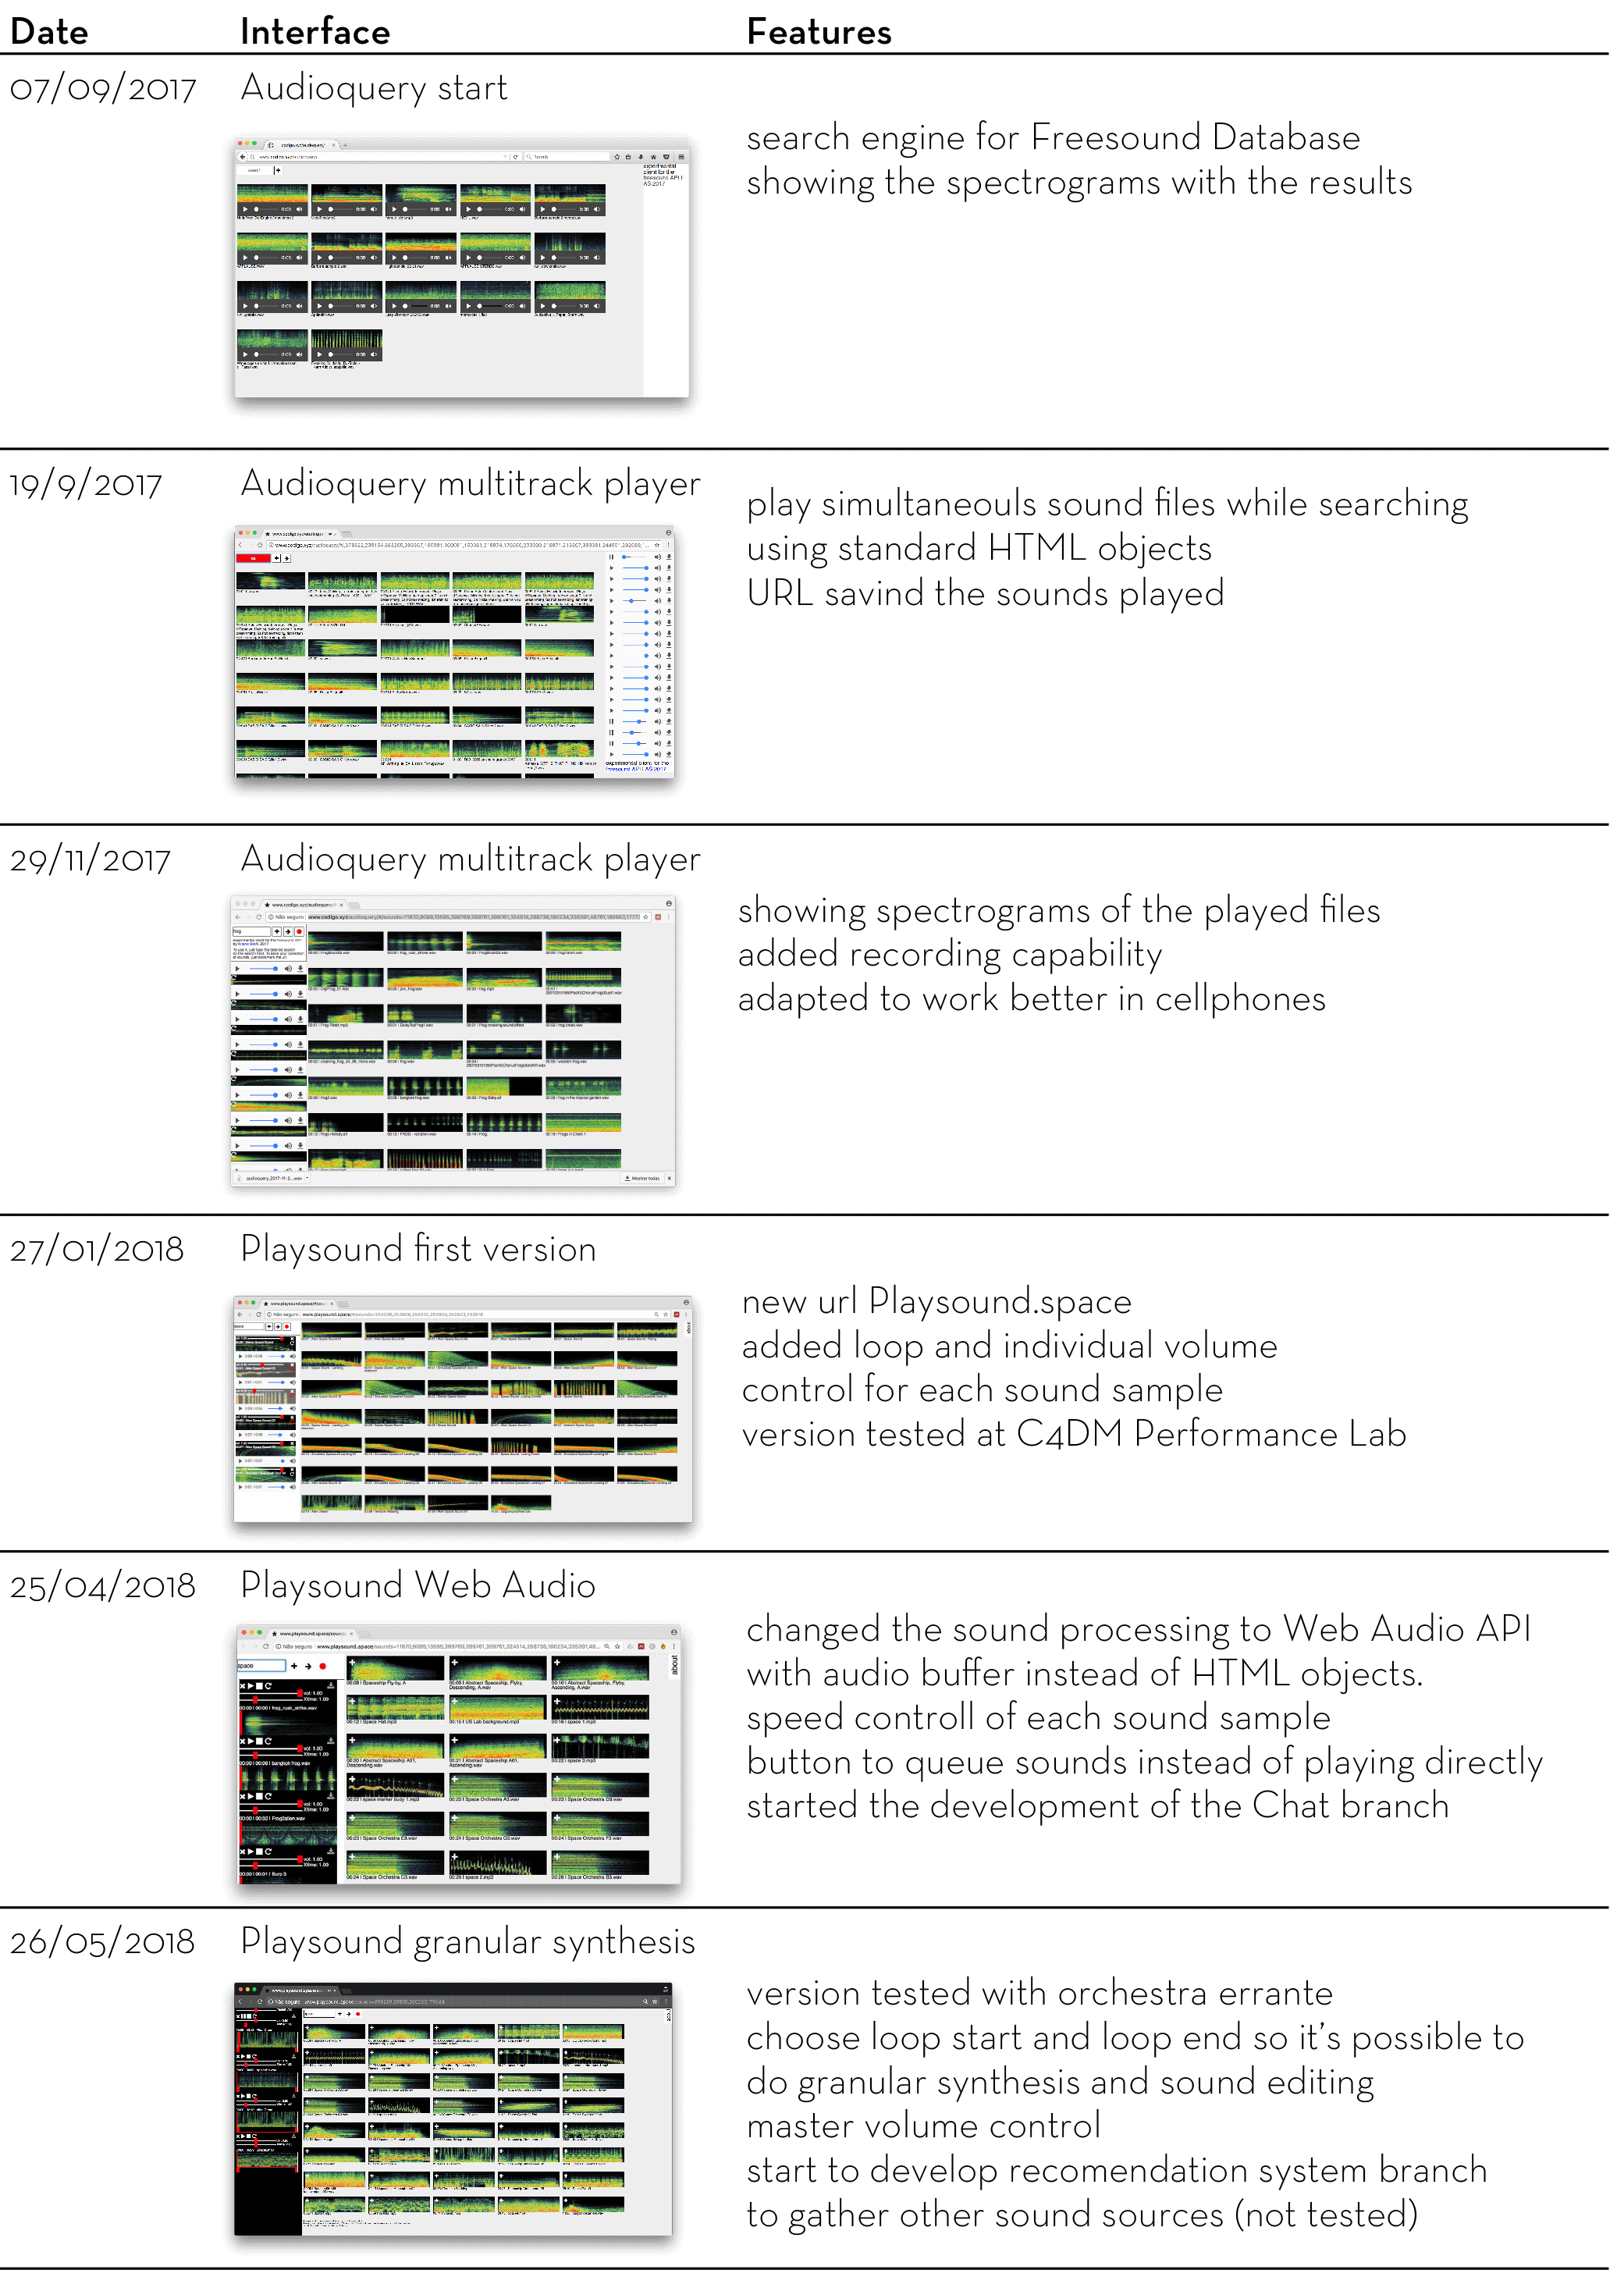
\includegraphics[width=0.8\textwidth]{pictures/playsoundtimeline}
\caption{\label{pstimeline}Playsound development timeline}
\label{fig:timeline}
\end{figure}

Comecei a desenvolver o projeto em Julho de 2018, após apresntar o Banda Aberta em alguns eventos na Europa que descrevi na seção anterior. A figura \ref{fig:timeline} apresenta os principais estágios de desenvolvimento da ferramenta de Setembro de 2017 a Julho de 2018. Utilizei novamente Lean Ux \cite{Liikkanen2014} como metodologia de desenvolvimento de software. Dentro dos princípios desse método, começamos novamente o projeto a partir de um protótipo bem simples, que era apenas um sistema de busca que mostrava o resultado como um conjunto de spectrogramas. Inicialmente, contei com a ajuda do programador Miguel Ceriani para fazer a ligação com a API do freesound.

Utilizamos como \emph{framework} Angular.js\footnote{Angular.js é um \emph{framework} em JavaScript desenvolvido pela Google que permite automatizar certos processos computacionais e facilita a comunicação com bancos de dados}. O Framework fornece o recurso de ligação de dados bidirecional, que faz com que a busca aconteça no servidor simultaneamente ao se digitar o texto na caixa de busca. Deste modo, mesmo antes de se completar uma palavra, resultados já começam a aparecer na janela do navegador. Para o processo de improvisação livre, esse recurso se mostrou muito interessante, uma vez que sons não esperados podem surgir mesmo antes de se estabelecer um vocábulo definitivo. 

Os resultados são apresentados na forma de spectrogramas, que permitem que o usuário do sistema tenha informações sobre ritmo e timbre das amostras recebidas antes de escolher o som para tocar. Os resultados são apresentados em uma matriz, que permite que se compare os sons visualmente. Apesar de a leitura dos spectrogramas não ser uma coisa corriqueira para qualquer usuário do sistema, acreditamos que um aprendizado implícito pode acontecer no simples processo de pesquisar e tocar com o sistema, quando se percebe a co-relação entre a representação gráfica das propriedades espectro-temporais dos dos sons e suas qualidades audíveis. Quando selecionamos uma imagem, o som é adicionado a uma playlist na lateral da interface.

 Assim que colocamos o sistema no ar, começamos a desenvolver recursos adicionais para transformar o sistema em um instrumento musical de fato. O primeiro recurso desenvolvido foi a capacidade de se fazer novas buscas enquanto os sons são tocados, recurso que já não existe no próprio Freesound. Em seguida, criamos um sistema de url para armazernar uma coleção de sons feita previamente. Cada som selecionado gera um código que fica registrado no endereço do navegador. Desta forma, é possível recuperar uma ``composição de sons'' para utilização futura. O próximp passo foi desenvolver a interface para tocar os arquivos. A primeira versão funcionava baseada em objetos HTML, utilizando o \emph{player} padrão dos navegadores para objetos de áudio que oferece controles apenas de pausar tocar, alterar o instante tocado e dependendo do navedagor um controle de volume. Em uma segunda versão utilizamos o tocador do Freesound, que oferecia recursos de loop, mas isso exigia que se recarregasse a página, interrompendo o fluxo musical. 

 Desenvolvemos alguns recursos básicos do tocador, adicionando a imagem do espectro sonoro como recurso mneumônico, e adicionamos controle individual de volume e loop para cada som que era adicionado à playlist. Como recurso de usabilidade, para dar feedback visual, a transparência da imagem é alterada conforme o volume do som aumenta ou abaixa. Adicionamos também um gravador embutido no sistema, que permite que as seções sejam gravadas em arquivos WAV. Esses arquivos podem ser salvos ou re-inseridos na interface para serem tocados. A figura \ref{fig:audioquery} mostra a interface da primeira versão do software no Google Chrome. \footnote{Por questões acadêmicas, mantemos ainda uma versão funcional do software em \url{http://www.codigo.xyz/audioquery/#/sounds=49333,415849}}.

\begin{figure}
\centering
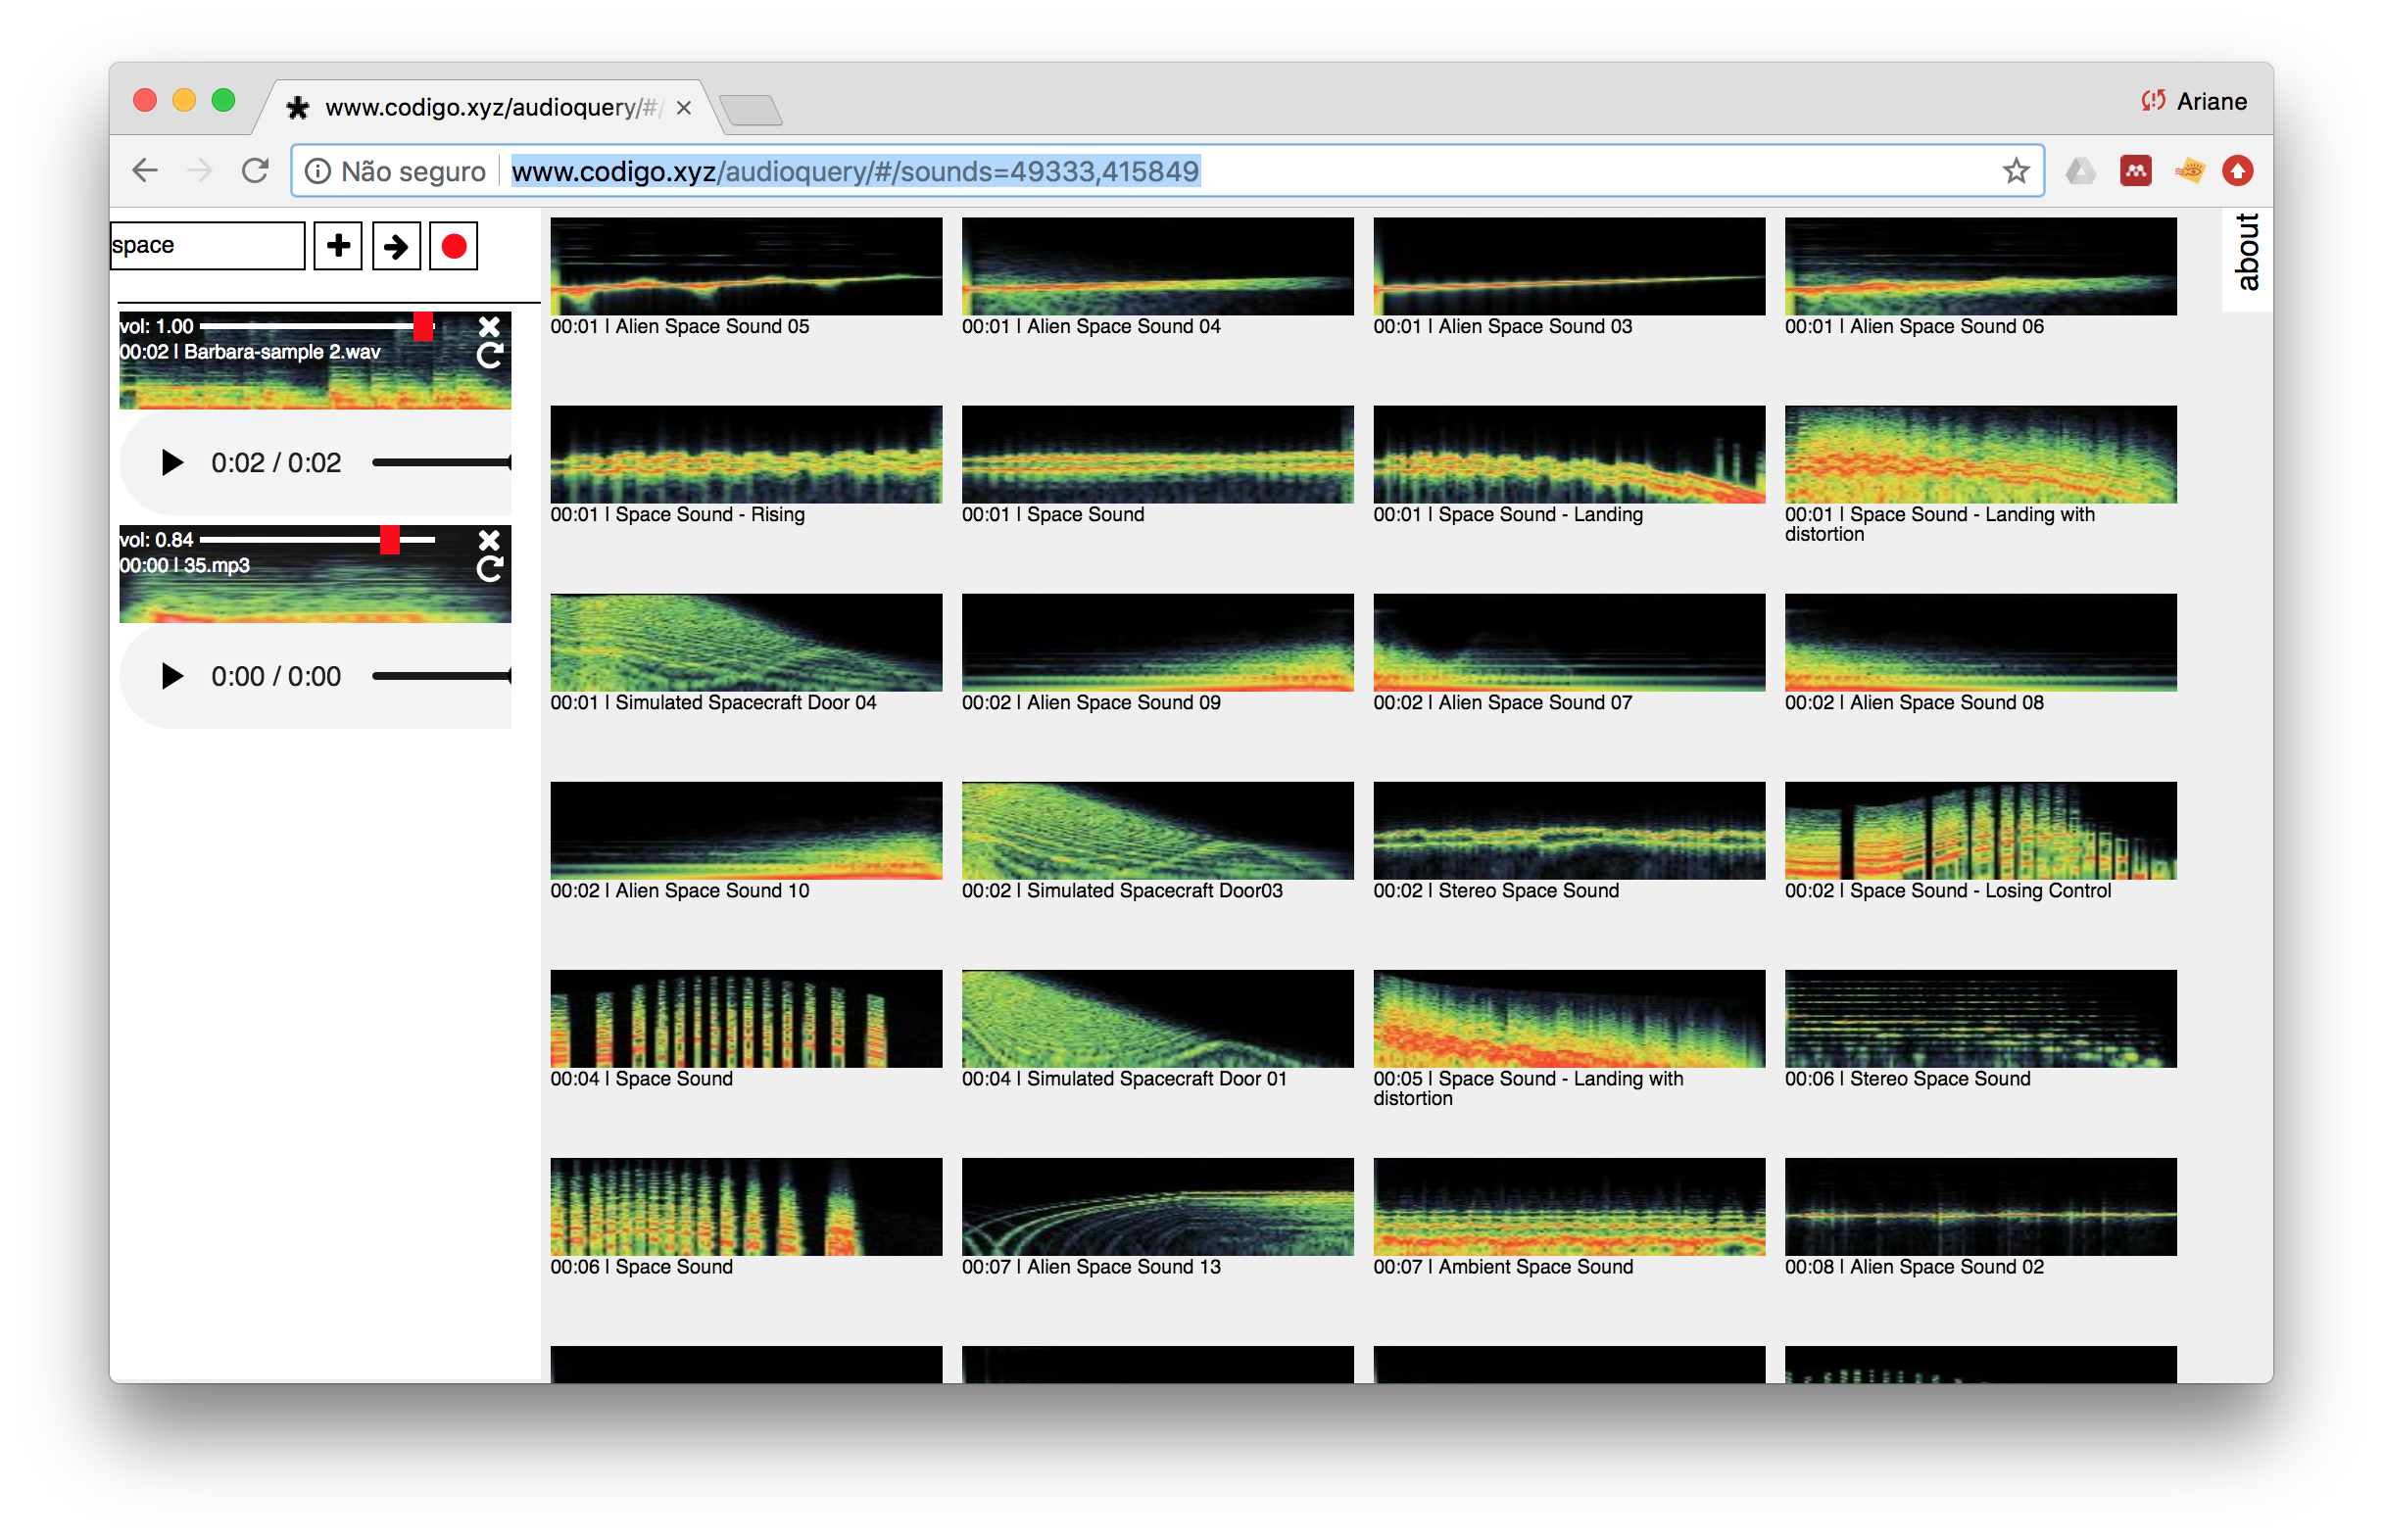
\includegraphics[width=0.8\textwidth]{pictures/cap4/audioquery}
\caption{\label{pstimeline}Primeira versão funcional do software desenvolvida.}
\label{fig:audioquery}
\end{figure}

 %Mais adiante, passei a contar com a ajuda da {}programadora Alessia Millo, que colaborou no desenvolvimento do tocador e de outros recursos que implantamos no sistema. Ela trabalhou na adaptação do sistema para utilizar as tecnologias de Web Audio, ao invés dos objetos HTML, que permitiu uma série de recursos que implementamos posteriormente, como a possibilidade de escolher o começo e o fim dos pontos de loop, alterar a velocidade de reprodução de sons e posição estéreo dos sons.




\end{otherlanguage*}

\phantomsection

